%%%%%%%%%%%%%%%%%%%%%%%%%%%%%%%%%%%%%%%%%%%%
\section{Looking inside the human body}

%%%%%%%%%%%%%%%%%%%%%%%%%%%%%%%%%%%%%%%%%%%%%%%%%%%%%%%%
{
%\paper{}
\begin{frame}{}

\BigSizeFont
\begin{center}
    Do you know \\
    how clinicians can actually monitor fetal development?
\end{center}


\end{frame}
}


%%%%%%%%%%%%%%%%%%%%%%%%%%%%%%%%%%%%%%%%%%%%%%%%%%%%%%%%
{
\paper{\faWikipediaW \hspace{1mm} \url{https://en.wikipedia.org/wiki/Medical_imaging_in_pregnancy}}
\begin{frame}{Computational Tomography}
      \begin{figure}
        \centering
        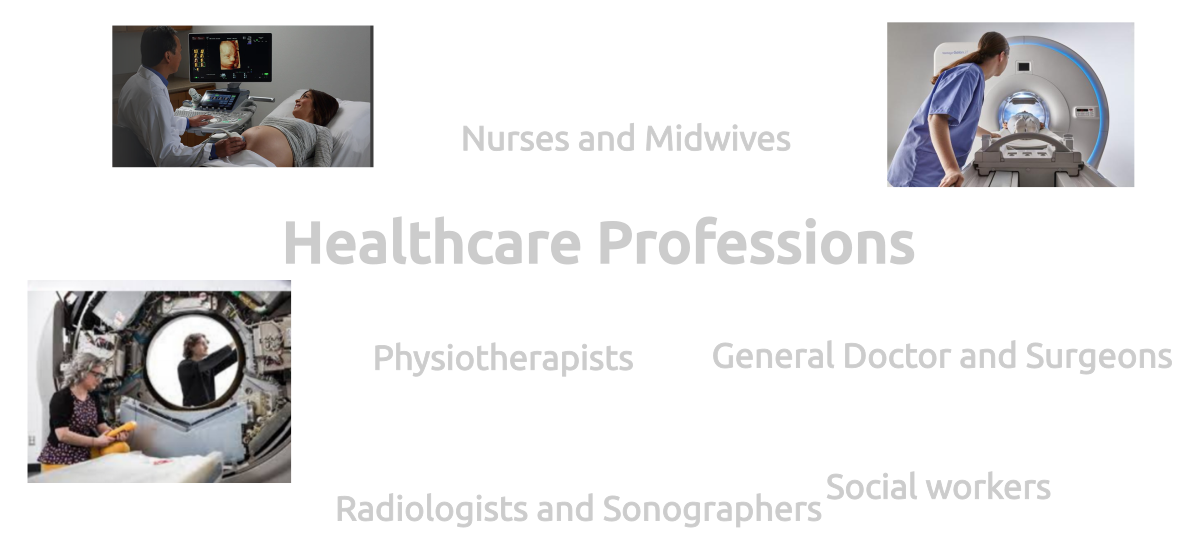
\includegraphics[width=1.0\textwidth]{./../figures/medical-imaging-in-pregnancy/ct/versions/drawing-v01.png}
        %\caption{}
      \end{figure}
\end{frame}
}


%%%%%%%%%%%%%%%%%%%%%%%%%%%%%%%%%%%%%%%%%%%%%%%%%%%%%%%%
{
\paper{\faWikipediaW \hspace{1mm} \url{https://en.wikipedia.org/wiki/Medical_imaging_in_pregnancy}}
\begin{frame}{Magnetic Resonance Imaging}
      \begin{figure}
        \centering
        \includegraphics[width=1.0\textwidth]{./../figures/medical-imaging-in-pregnancy/mri/versions/drawing-v00.png}
        %\caption{}
      \end{figure}
\end{frame}
}


%%%%%%%%%%%%%%%%%%%%%%%%%%%%%%%%%%%%%%%%%%%%%%%%%%%%%%%%
{
\paper{\faWikipediaW \hspace{1mm} \url{https://en.wikipedia.org/wiki/Medical_imaging_in_pregnancy}}
\begin{frame}{Ultrasound}
      \begin{figure}
        \centering
        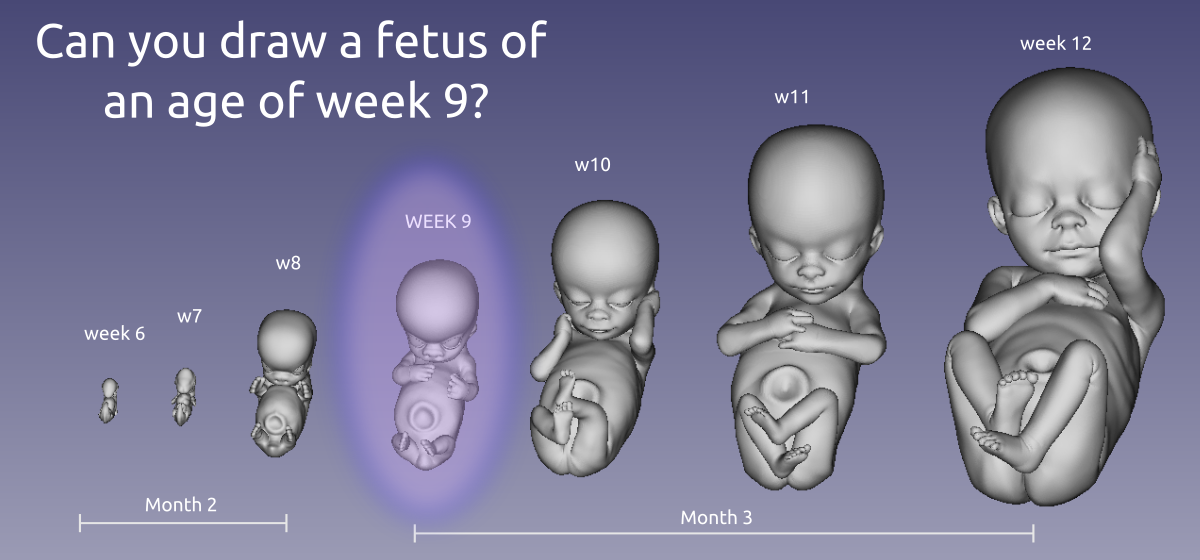
\includegraphics[width=1.0\textwidth]{./../figures/medical-imaging-in-pregnancy/us/versions/drawing-v02.png}
        %\caption{}
      \end{figure}
\end{frame}
}

%%%%%%%%%%%%%%%%%%%%%%%%%%%%%%%%%%%%%%%%%%%%%
%\subsection{FETUS}
%Medical imaging in pregnancy

%%%%%%%%%%%%%%%%%%%%%%%%%%%%%%%%%%%%%%%%%%%%%%%%%%%%%%%%
{
\paper{\faWikipediaW \hspace{1mm} \url{https://en.wikipedia.org/wiki/Medical_imaging_in_pregnancy}}
\begin{frame}{Medical Imaging in Pregnancy}
      \begin{figure}
        \centering
        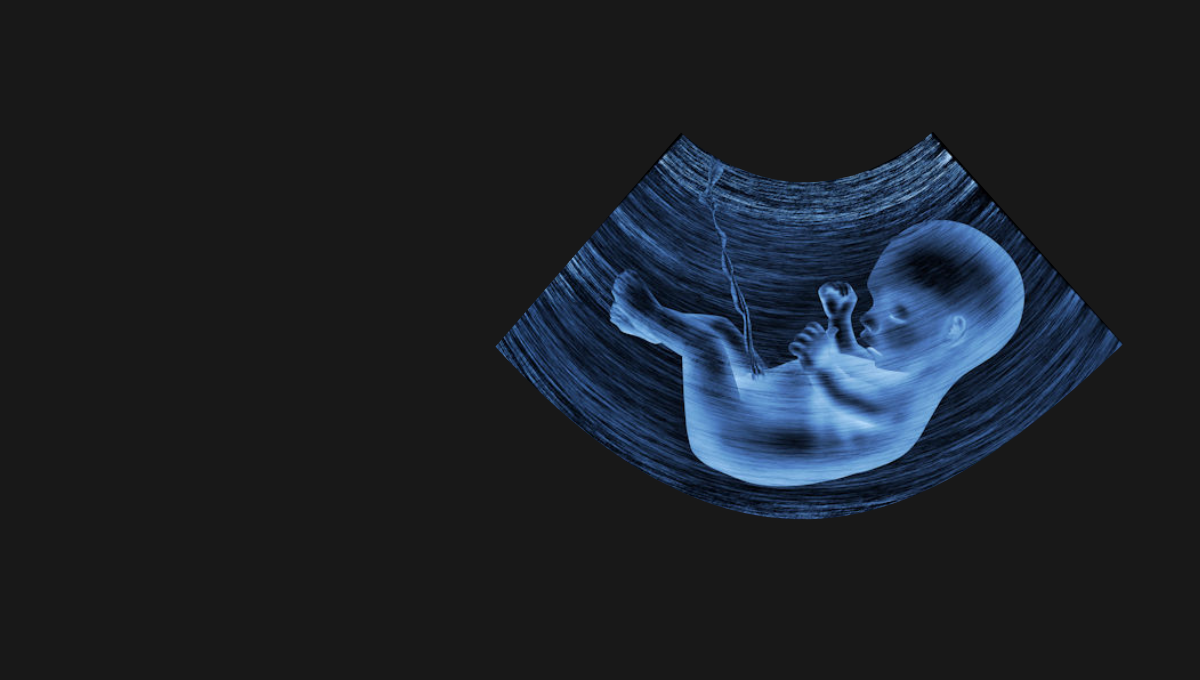
\includegraphics[width=1.0\textwidth]{./../figures/medical-imaging-in-pregnancy/ct-mr-us/versions/drawing-v03.png}
        %\caption{}
      \end{figure}
\end{frame}
}



%{ % all template changes are local to this group.
%    \setbeamertemplate{navigation symbols}{}
%    \begin{frame}<article:0>[plain]
%        \begin{tikzpicture}[remember picture,overlay]
%            \node[at=(current page.center)] {
%                \includegraphics[keepaspectratio,
%                                 width=\paperwidth,
%                                 height=\paperheight]{./figures/medical-imaging-in-pregnancy/us/versions/drawing-v00.png}
%            };
%        \end{tikzpicture}
%     \end{frame}
%}

